\chapter{Introducing an Augmented Model}
\label{chap:augmentedmodel}

The evaluation in Chapter~\ref{chap:evaluation} reveals that the arbitrage-free encoder--decoder model struggles to reconstruct negative-rate and inverted curves, which are curve types that are underrepresented in the training data. This chapter addresses that limitation. We propose the so-called \textit{augmented} model, which modifies the input representation to provide the encoder with additional information about curve shape, with the aim of improving reconstruction for curve types underrepresented in training data. Throughout the remainder of this chapter and the rest of the thesis, the original encoder--decoder of \citet{MatinWanPoulsen2025}, as introduced in Chapter~\ref{chap:encoderdecodermodel}, is referred to as the \textit{baseline} model.

\section{Motivating Augmentation}
\label{sec:model_aug}

When the baseline model is trained on the full sample period over 5\,000 epochs, two distinct failure patterns emerge for \textit{negative} curves. For \textit{deeply negative} curves the model reconstructs a curve sloping in the wrong direction entirely. For \textit{crossing} curves the model instead produces a flat curve near zero, capturing the level but missing the slope entirely. 
Beyond these two patterns, inverted curves are also reconstruced poorly, with the model failing to capture both the short and long ends, lacking sufficient curvature and slope. These three curve types are defined in Table \ref{tab:curve_type_counts} (Chapter \ref{chap:datadescription}). All three patterns are illustrated in Figure~\ref{fig:baseline_fit_failure_modes}, alongside a well-reconstructed \textit{normal} curve included as a benchmark for accurate reconstruction.

\begin{figure}[h]
    \centering
    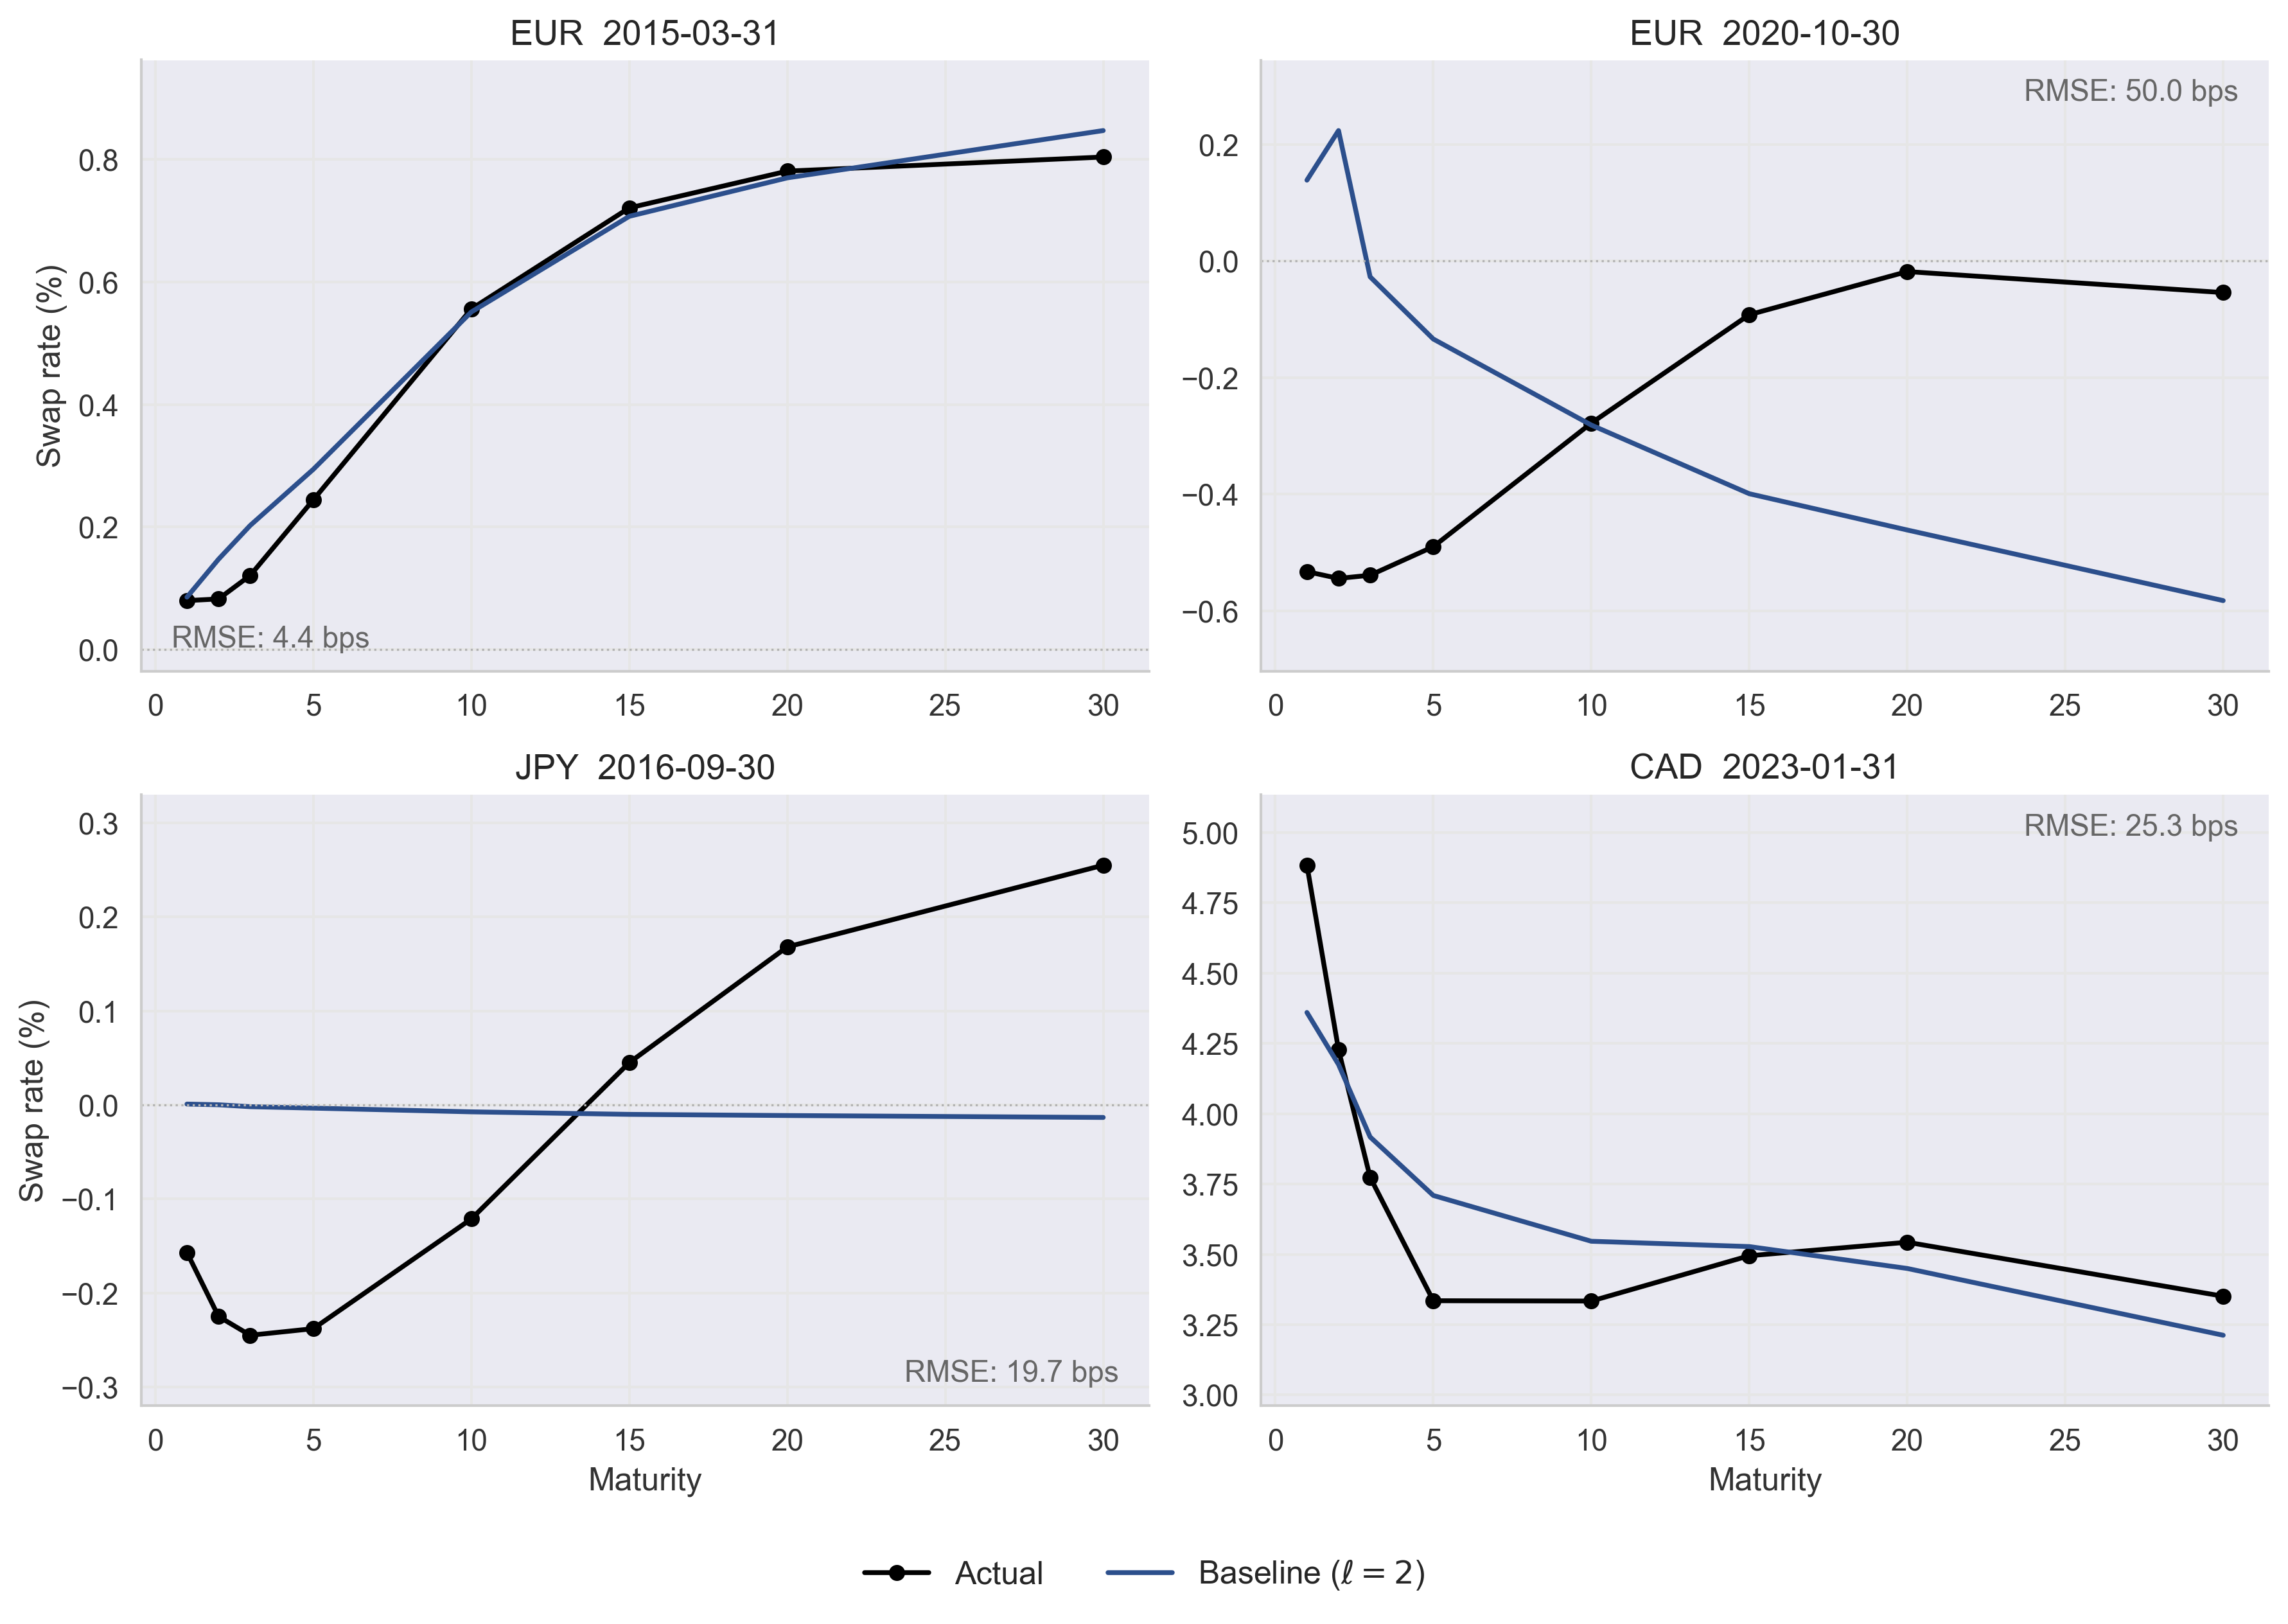
\includegraphics[width=\textwidth]{Figures/thesis_results/AutoencoderPerformanceAugmented/baseline_fit_failure_modes.png}
    \caption{Baseline ($\ell = 2$) reconstruction for four representative swap curves. The normal EUR curve (2015-03-31) is reconstructed accurately and serves as a reference case. The remaining three panels illustrate the in-sample failure patterns: the deeply negative EUR curve (2020-10-30) and the crossing JPY curve (2016-09-30) show the two distinct failures for negative-rate curves, and the inverted CAD curve (2023-01-31) shows the failure for inverted curves. In-sample RMSE is annotated in each panel.}
    \label{fig:baseline_fit_failure_modes}
\end{figure}

As concluded in Chapter~\ref{chap:evaluation}, these patterns persist regardless of the number of latent factors, suggesting that the issue lies not in the dimensionality of the latent space but elsewhere. 

We hypothesise that this is linked to the linearity of the encoder. Specifically, since $z = A_1\mathbf{S}$ is a linear map with no bias or activation function and $A_1$ is trained on data dominated by positive-rate curves, the latent states produced by negative-rate curves lie outside the distribution seen during training, resulting in poor reconstruction of these curve types. We illustrate this through the following examples.

\begin{example}\label{ex:level}
Consider the two EUR swap curves visible in Figure~\ref{fig:baseline_fit_failure_modes}, $\mathbf{S}^{+}$ with positive rates and $\mathbf{S}^{-}$ with negative rates, both sharing the same upward-sloping 
shape. Holding the curve shape fixed, we additionally construct 
$\mathbf{S}^{\text{shift}}$ by shifting $\mathbf{S}^{-}$ upward by $0.0061$, bringing it to the same starting level as 
$\mathbf{S}^{+}$,
\begin{align*}
\mathbf{S}^{+} = \begin{pmatrix} 0.0008 \\ 0.0008 \\ 0.0012 \\ 0.0024 \\ 0.0056 \\ 
0.0072 \\ 0.0078 \\ 0.0080 \end{pmatrix}, \qquad
\mathbf{S}^{-} = \begin{pmatrix} -0.0053 \\ -0.0054 \\ -0.0054 \\ -0.0049 \\ 
-0.0028 \\ -0.0009 \\ -0.0002 \\ -0.0005 \end{pmatrix}, \qquad
\mathbf{S}^{\text{shift}} = \begin{pmatrix} 0.0008 \\ 0.0007 \\ 0.0007 \\ 0.0012 \\ 
0.0033 \\ 0.0052 \\ 0.0059 \\ 0.0056 \end{pmatrix}.
\end{align*}
That all three curves slope upward is reflected in their short-end slope features, 
defined as the difference between the $10$Y and $1$Y tenors,
\begin{align*}
    f_1^{+} = 0.0056 - 0.0008 = 0.0048\\
    f_1^{-} = -0.0028 - (-0.0053) = 0.0025\\
    f_1^{\text{shift}} = 0.0033 - 0.0008 = 0.0025
\end{align*}
which are all positive and of similar magnitude.

The learned encoder matrix for the $\ell=2$ baseline model, trained on the full sample and therefore predominantly on positive-rate curves (see Table~\ref{tab:curve_type_counts}), is
$$A_1 = \begin{pmatrix} 0.46 & 0.37 & 0.00 & 0.40 & 0.26 & -0.23 & -0.66 & -0.10 \\ 
-1.12 & -0.63 & -0.66 & -0.83 & -0.50 & -0.29 & -0.22 & 0.13 \end{pmatrix}.$$ 
which yields the latent representations
$$z^{+} = A_1\mathbf{S}^{+}=\begin{pmatrix} -0.0045 \\ -0.0098 \end{pmatrix}, \qquad
z^{-} = A_1\mathbf{S}^{-}=\begin{pmatrix} -0.0068 \\ +0.0186 \end{pmatrix}, \qquad
z^{\text{shift}} = A_1\mathbf{S}^{\text{shift}}=\begin{pmatrix} -0.0036 \\ -0.0065 \end{pmatrix}.$$
Despite $\mathbf{S}^{-}$ and $\mathbf{S}^{\text{shift}}$ having identical shapes, their latent representations lie in very different regions of the latent space. The shifted curve lands close to $\mathbf{S}^{+}$, with $\|z^{+} - z^{\text{shift}}\| = 0.0034$, while the negative-rate curve is mapped far away, with $\|z^{+} - z^{-}\| = 0.0284$, roughly eight times further. The encoder therefore separates curves by their rate level rather than their shape.\;\;$\circ$
\end{example}


To further quantify the encoder's sensitivity to level versus shape, Example~\ref{ex:level_shape_entanglement} compares the latent displacement caused by equal-magnitude level and slope perturbations.



\begin{example}\label{ex:level_shape_entanglement}
Continuing with the positive-rate curve $\mathbf{S}^{+}$ and encoder matrix $A_1$ 
from Example~\ref{ex:level}, we compare the latent displacement caused by a parallel level shift with that caused by a slope change. To ensure a fair comparison, we require the two input perturbations to have the same Euclidean norm.

Define the level perturbation vector $\mathbf{1} = (1,\ldots,1)^\top \in \mathbb{R}^8$ and the slope perturbation vector $\mathbf{v} = (-1,-1,-1,-1,1,1,1,1)^\top \in \mathbb{R}^8$ so that $\|\mathbf{1}\| = \|\mathbf{v} \| = \sqrt{8}$. Then for any scalar $c \in \mathbb{R}$, the perturbations $c\mathbf{1}$ and $c\mathbf{v} $ have equal Euclidean norm $|c|\sqrt{8}$.

For a parallel level shift of magnitude $c$, define
\[
\mathbf{S}^{\text{level}} = \mathbf{S}^{+} + c\mathbf{1},
\]
which shifts all tenors by $c$. By linearity of the encoder, the resulting 
displacement in the latent space is
\[
\Delta z_{\text{level}} := A_1\mathbf{S}^{\text{level}} - A_1\mathbf{S}^{+} = cA_1\mathbf{1}.
\]
Since $A_1\mathbf{1} = (0.50, -4.12)^\top$, setting $c = 0.01$ yields
\[
\Delta z_{\text{level}} = (0.0050, -0.0412)^\top, \qquad 
\|\Delta z_{\text{level}}\| \approx 0.0415.
\]
For a slope change of the same magnitude, define
\[
\mathbf{S}^{\text{slope}} = \mathbf{S}^{+} + c\mathbf{v} ,
\]
which lowers the short end by $c$ and raises the long end by $c$, introducing no net level change since the entries of $\mathbf{v} $ sum to zero. The displacement 
in the latent space is
\[
\Delta z_{\text{slope}} := A_1\mathbf{S}^{\text{slope}} - A_1\mathbf{S}^{+} = cA_1\mathbf{v} .
\]
Since $A_1\mathbf{v}  = (-1.96, 2.36)^\top$, we obtain
\[
\Delta z_{\text{slope}} = (-0.0196, 0.0236)^\top, \qquad 
\|\Delta z_{\text{slope}}\| \approx 0.0307.
\]
Under equal-norm input perturbations, the level shift produces a latent 
displacement approximately $0.0415 / 0.0307 \approx 1.35$ times larger than 
the slope change, suggesting that the encoder is more sensitive to the absolute level of rates than to the shape of the curve.\;\;$\circ$
\end{example}

Together, Examples~\ref{ex:level} and~\ref{ex:level_shape_entanglement} illustrate that the linear encoder is more sensitive to the rate level than to the curve shape, mapping geometrically similar curves to very different regions of the latent space when their rate levels differ in sign, with a level shift producing roughly 1.35 times the latent displacement of an equal-magnitude slope change. Given the linearity of the encoder, we hypothesise that this extends beyond negative-rate curves to any curve type underrepresented in training.



Figure~\ref{fig:prevalence_baseline} shows the result of training the baseline model at different shares of negative-rate curves and evaluating reconstruction accuracy on two fixed sets of curves withheld from training, one consisting solely of negative-rate curves and one of normal-rate curves. The model reconstructs best whichever curve type it sees most in training. As the share of negative-rate curves increases, their RMSE decreases monotonically, while normal-rate RMSE rises. The two series cross at approximately 50\%, where the training set consists of equal shares of negative-rate and normal-rate curves and both evaluation sets yield similar errors, confirming that reconstruction accuracy is governed by representation in the training data, not by any inherent difficulty of one curve type over the other.

\begin{figure}[H]
    \centering
    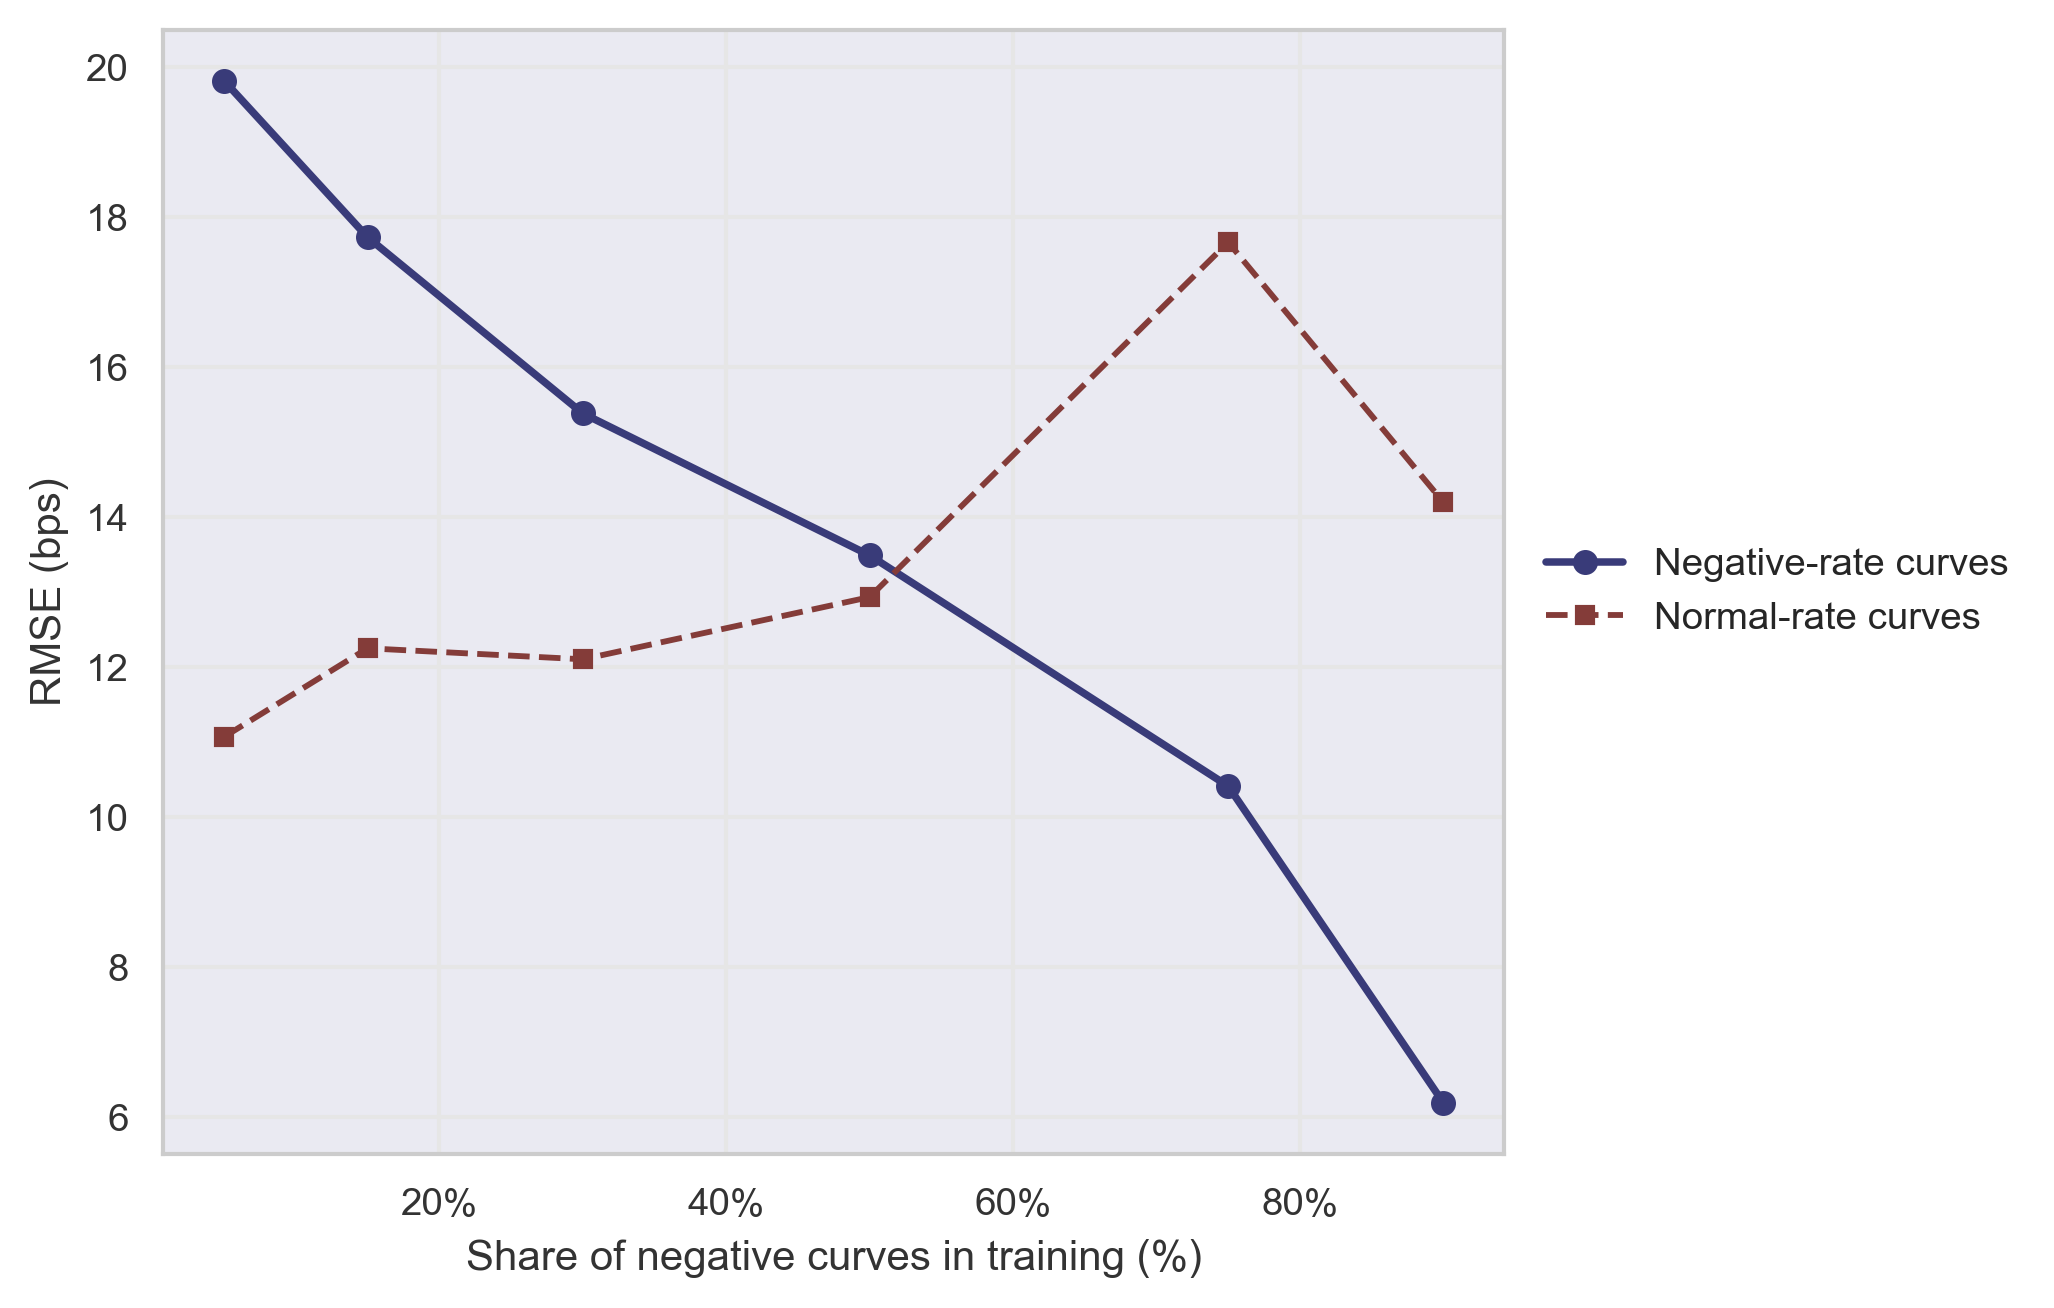
\includegraphics[width=0.75\textwidth]{Figures/Experiments/PrevalenceSweep/plots_dim2_ep3500_N1500/prevalence_baseline_only.png}
    \caption{RMSE (bps) as a function of the share of negative-rate curves in the training set, for the baseline model ($\ell = 2$). Each point represents a trained model evaluated on a fixed set of negative-rate curves withheld from training (solid line) and a fixed set of normal-rate curves withheld from training (dashed line). The monotone decrease in negative-rate RMSE and corresponding increase in normal-rate RMSE as the share increases suggests that reconstruction accuracy is governed by representation in the training data rather than by any inherent difficulty of the curve type.}
    \label{fig:prevalence_baseline}
\end{figure}


The examples and the representation experiment together suggest that poor reconstruction of underrepresented curve types stems from the linear encoder mapping them to unexplored regions of the latent space, not from any inherent difficulty of those shapes. This motivates augmenting the input with slope and curvature features, giving the encoder shape information that is more independent of rate level. The augmented model is the subject of the following section.



\section{The Augmented Model}

To make the shape of the curve more explicit when fed to the encoder, we augment the input vector with three derived features. Following the notation of Chapter~\ref{chap:encoderdecodermodel}, $S^{(i)}$ denotes the par swap rate at maturity $\tau_i$, and we define a \(b= \left\lceil \frac{M}{2}\right\rceil +1\), such that \(\tau = \tau_1, \dotsc, \tau_b, \dots, \tau_M\). We define a short-end slope $f_1$, a long-end slope $f_2$, and a 
curvature measure $f_3$ as
\[
f_1 = S^{(b)} - S^{(1)}, \qquad f_2 = S^{(M)} - S^{(b)}, \qquad 
f_3 = 2S^{(b)} - S^{(1)} - S^{(M)}.
\]
The augmented input vector is then defined as
\[
\mathbf{S}^{\text{aug}} = \bigl(S^{(1)}, \ldots, S^{(M)}, f_1, f_2, f_3\bigr)^\top 
\in \mathbb{R}^{M+3}.
\]
No new information is introduced by this augmentation, since the three features are deterministic functions of the rates already present in $\mathbf{S}$. The augmentation simply makes certain structural properties of the curve more explicit as inputs to the encoder.

A useful property of the derived features is that they are invariant to parallel level shifts. For any constant $c \in \mathbb{R}$, adding $c$ to swap rates for all maturities leaves the features unchanged,
\begin{align*}
\bar{f}_1 &= (S^{(b)} + c) - (S^{(1)} + c) = S^{(b)} - S^{(1)} = f_1, \\
\bar{f}_2 &= (S^{(M)} + c) - (S^{(b)} + c) = S^{(M)} - S^{(b)} = f_2, \\
\bar{f}_3 &= 2(S^{(b)} + c) - (S^{(1)} + c) - (S^{(M)} + c) = 2S^{(b)} - S^{(1)} - S^{(M)} = f_3.
\end{align*}

Since the slope and curvature features are defined as differences between maturity rates, the common level component cancels out exactly, making them invariant to parallel shifts in the rate curve and directly addressing the level sensitivity of the linear encoder illustrated in Examples~\ref{ex:level} and~\ref{ex:level_shape_entanglement}.

The augmented model is trained within the same encoder--decoder framework 
as described in Chapter~\ref{chap:encoderdecodermodel}, subject to two modifications. First, the encoder receives the augmented input $\mathbf{S}^{\text{aug}} \in \mathbb{R}^{M+3}$ 
rather than the swap curve $\mathbf{S} \in \mathbb{R}^{M}$, while the decoder still outputs an $M$-dimensional swap curve $\widetilde{\mathbf{S}}$. The shape features are then derived from $\widetilde{\mathbf{S}}$ in the same way as from $\mathbf{S}$, yielding the reconstructed augmented vector $\widetilde{\mathbf{S}}^{\text{aug}} \in \mathbb{R}^{M+3}$.

Second, the loss function 
is extended to penalise errors in the derived features in addition to the raw rates, yielding the empirical risk
\begin{equation}
\mathcal{L}^{\text{aug}}(\Omega) = \frac{1}{N(M + 3)} \sum_{n=1}^{N} 
\left\| \mathbf{S}_n^{\text{aug}} - \widetilde{\mathbf{S}}_n^{\text{aug}}(\Omega) 
\right\|^2,
\end{equation}

By including the derived features in the loss, the  model is penalised not only for errors in the raw rates but also for errors in the slope and curvature of the reconstructed curve, with all $M+3$ terms entering with equal weight. 


\section{Empirical Assessment}

Compared to the baseline, the augmented model improves reconstruction of underrepresented curve types when trained on the full sample, though the degree of improvement varies with the number of latent dimensions $\ell$. As seen in the top left panel of Figure~\ref{fig:failure_modes_all_models}, both models produce a close fit for the positive-rate EUR curve, establishing that the augmentation does not disturb performance on well-behaved curves.

\begin{figure}[H]
    \centering
    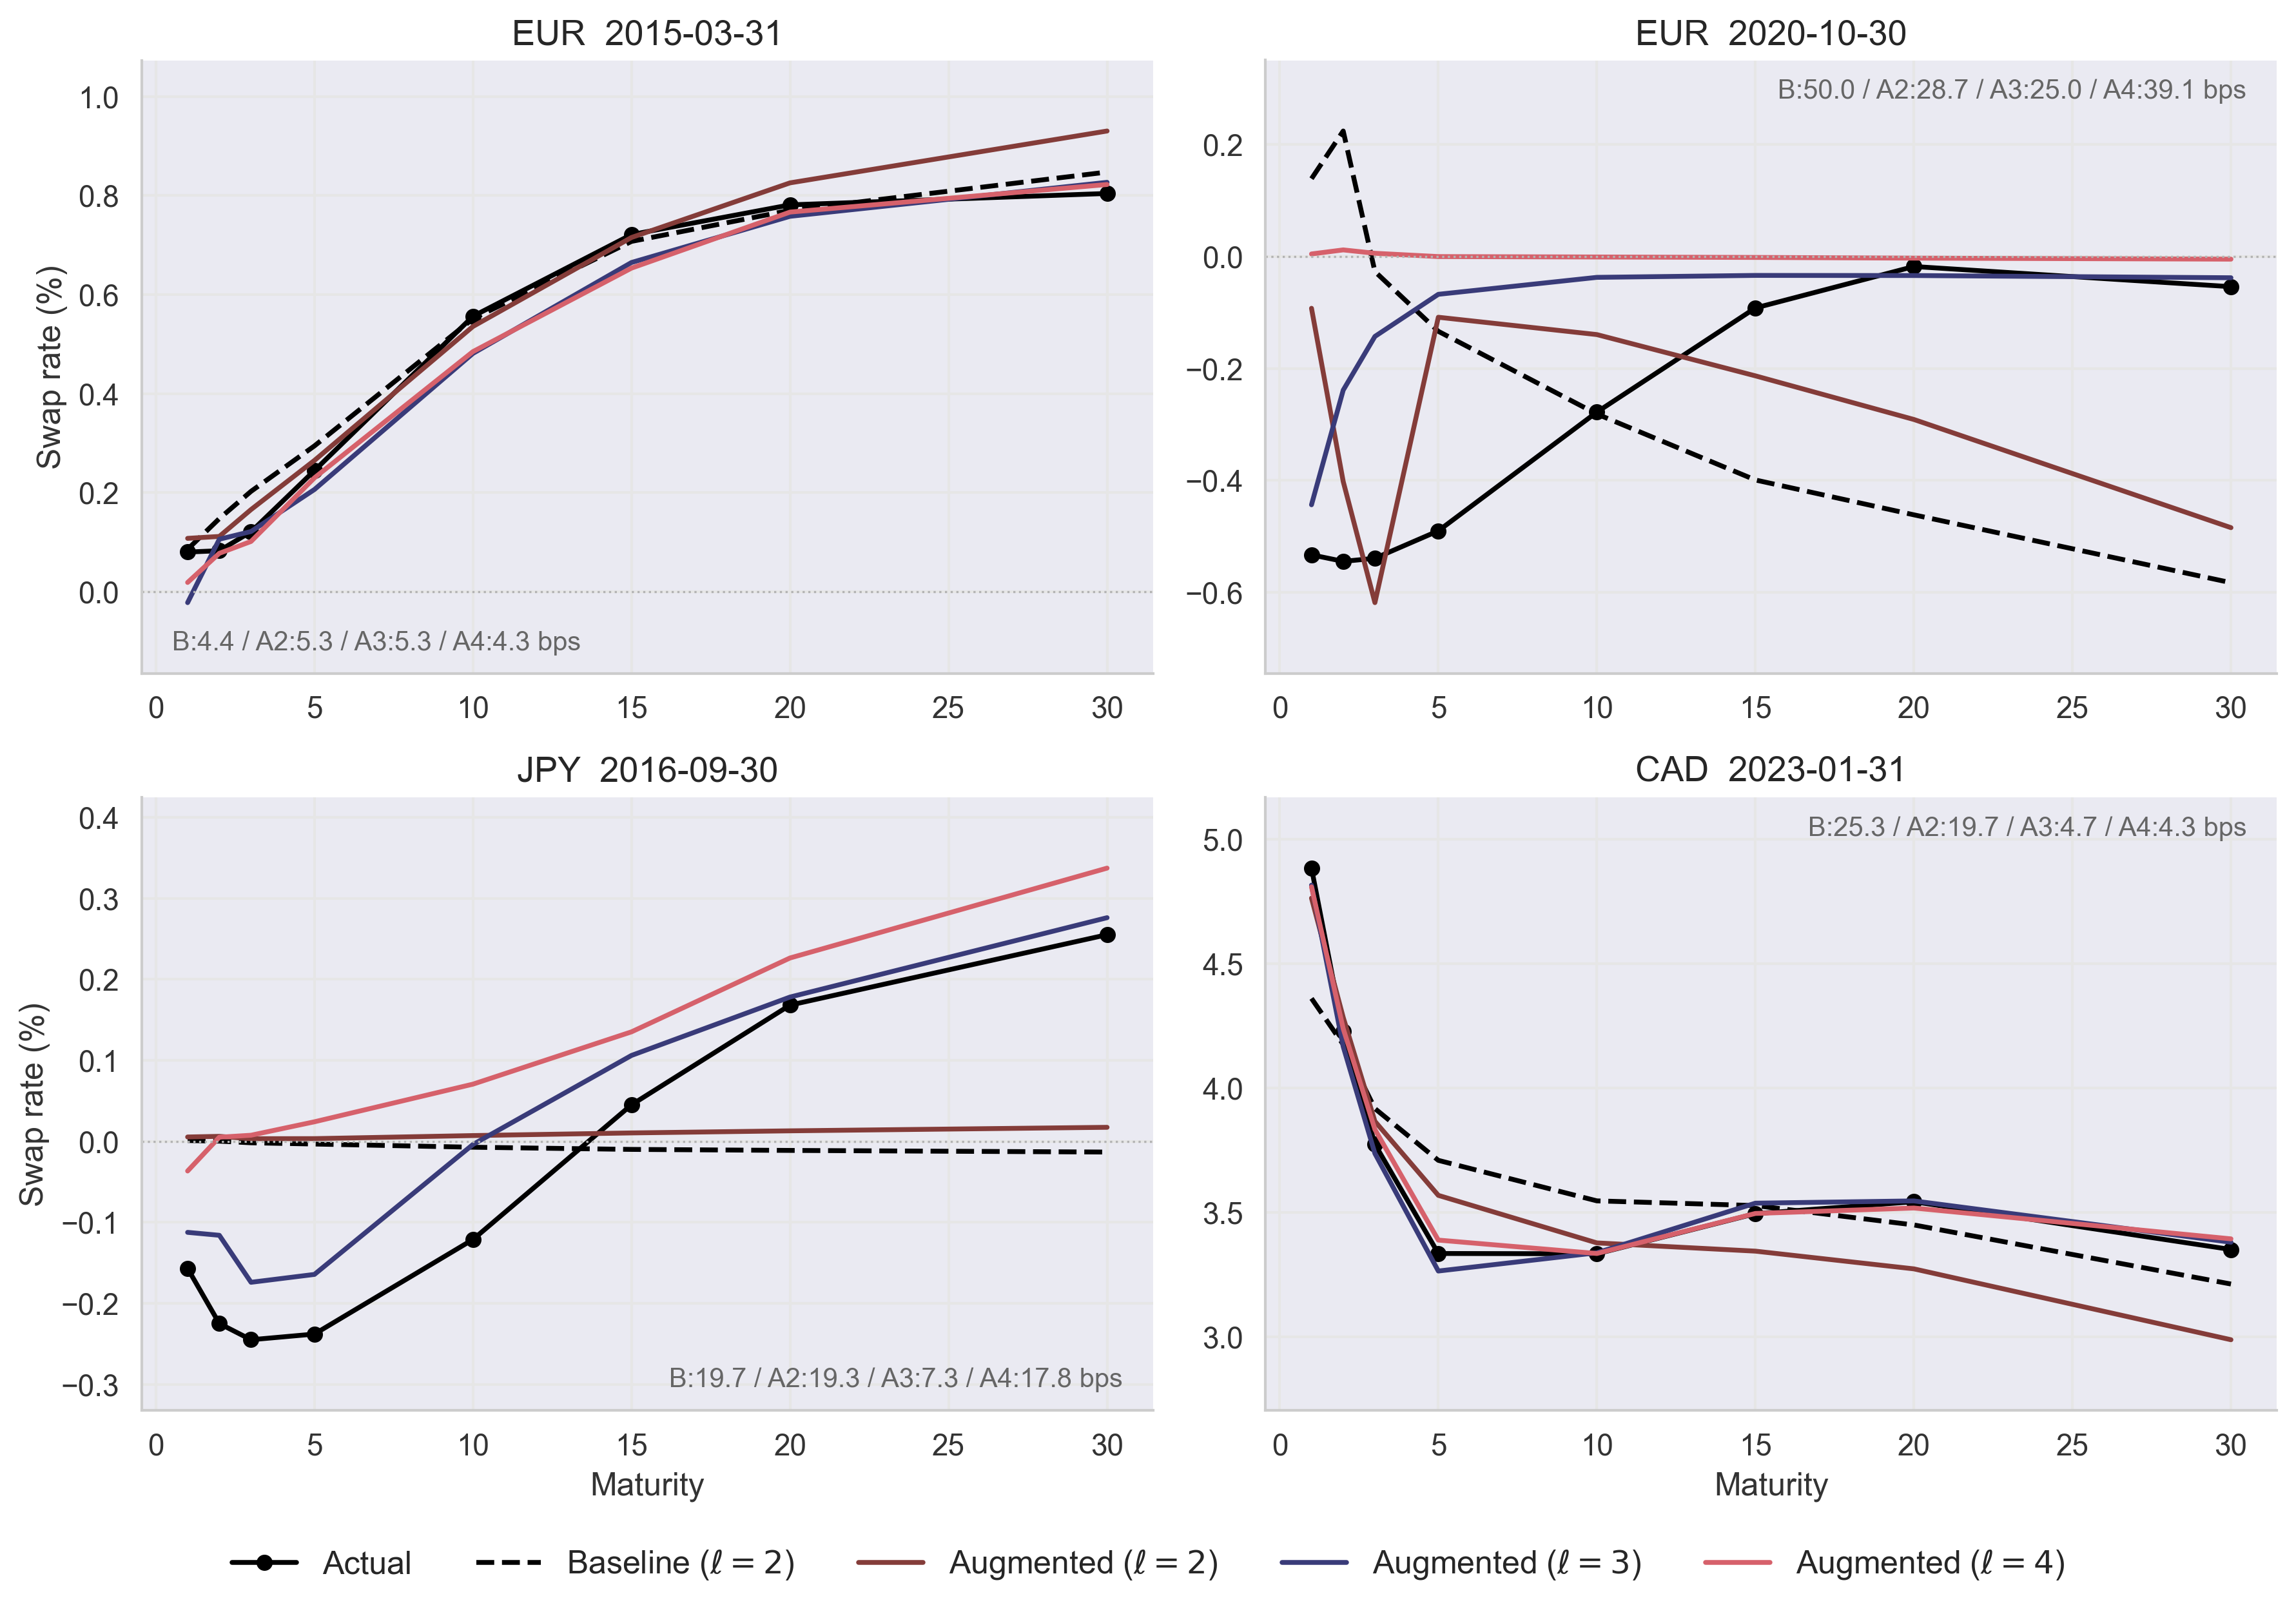
\includegraphics[width=0.95\textwidth]{Figures/thesis_results/AutoencoderPerformanceAugmented/failure_modes_all_models.png}
    %\caption{Baseline and augmented model reconstructions for four representative swap curves. \textit{Top left:} EUR 2015-03-31, a normal curve reconstructed accurately by all models. \textit{Top right:} EUR 2020-10-30, a deeply negative curve. \textit{Bottom left:} JPY 2016-09-30, a crossing curve with a negative short end and positive long end. \textit{Bottom right:} CAD 2023-01-31, an inverted curve. RMSE values (bps) are annotated as $\mathrm{B}$ (baseline, $\ell=2$), $\mathrm{A2}$ (augmented, $\ell=2$), $\mathrm{A3}$ (augmented, $\ell=3$), and $\mathrm{A4}$ (augmented, $\ell=4$).}
    \caption{Baseline and augmented model reconstructions for four representative swap curves. \textit{Top left:} EUR 2015-03-31, a normal curve reconstructed accurately by all models. \textit{Top right:} EUR 2020-10-30, a deeply negative curve. \textit{Bottom left:} JPY 2016-09-30, a crossing curve with a negative short end and positive long end. \textit{Bottom right:} CAD 2023-01-31, an inverted curve. RMSE values (bps) are annotated as $\mathrm{B}$ (baseline, $\ell=2$), $\mathrm{A2}$ (augmented, $\ell=2$), $\mathrm{A3}$ (augmented, $\ell=3$), and $\mathrm{A4}$ (augmented, $\ell=4$). The augmented model improves reconstruction for the negative-rate and inverted curves, while accuracy on the normal curve is maintained.}
    \label{fig:failure_modes_all_models}
\end{figure}

For the two negative-rate failure patterns the picture is more nuanced. The deeply negative EUR curve on 2020-10-30 remains challenging across all latent dimensions $\ell$. While the augmented models reconstruct the correct direction rather than producing a curve sloping the wrong way, they overshoot significantly at the short end. The best-performing specification, $\ell=3$, reduces the RMSE from approximately 50 to 25 basis points, a meaningful reduction that nonetheless remains a poor fit.

The crossing JPY curve on 2016-09-30 tells a more encouraging story: the augmented model at $\ell=3$ improves the fit, better capturing the upward slope from negative short-end rates to positive long-end rates. At $\ell=2$ the augmented model remains close to the baseline, while at $\ell=4$ it overshoots at the long end. For the inverted CAD curve on 2023-01-31, the augmented model at $\ell=3$ and 
$\ell=4$ improves the fit substantially relative to the baseline, reducing the 
RMSE from 25.3 to 4.7 and 4.3 basis points respectively, better capturing the 
curvature, while $\ell=2$ continues to mimic the baseline reconstruction. 

Across all three underrepresented curve types, the augmented model at $\ell=2$ performs similarly to the baseline, while improvements in slope and curvature become visible at $\ell=3$.

\begin{figure}[h]
    \centering
    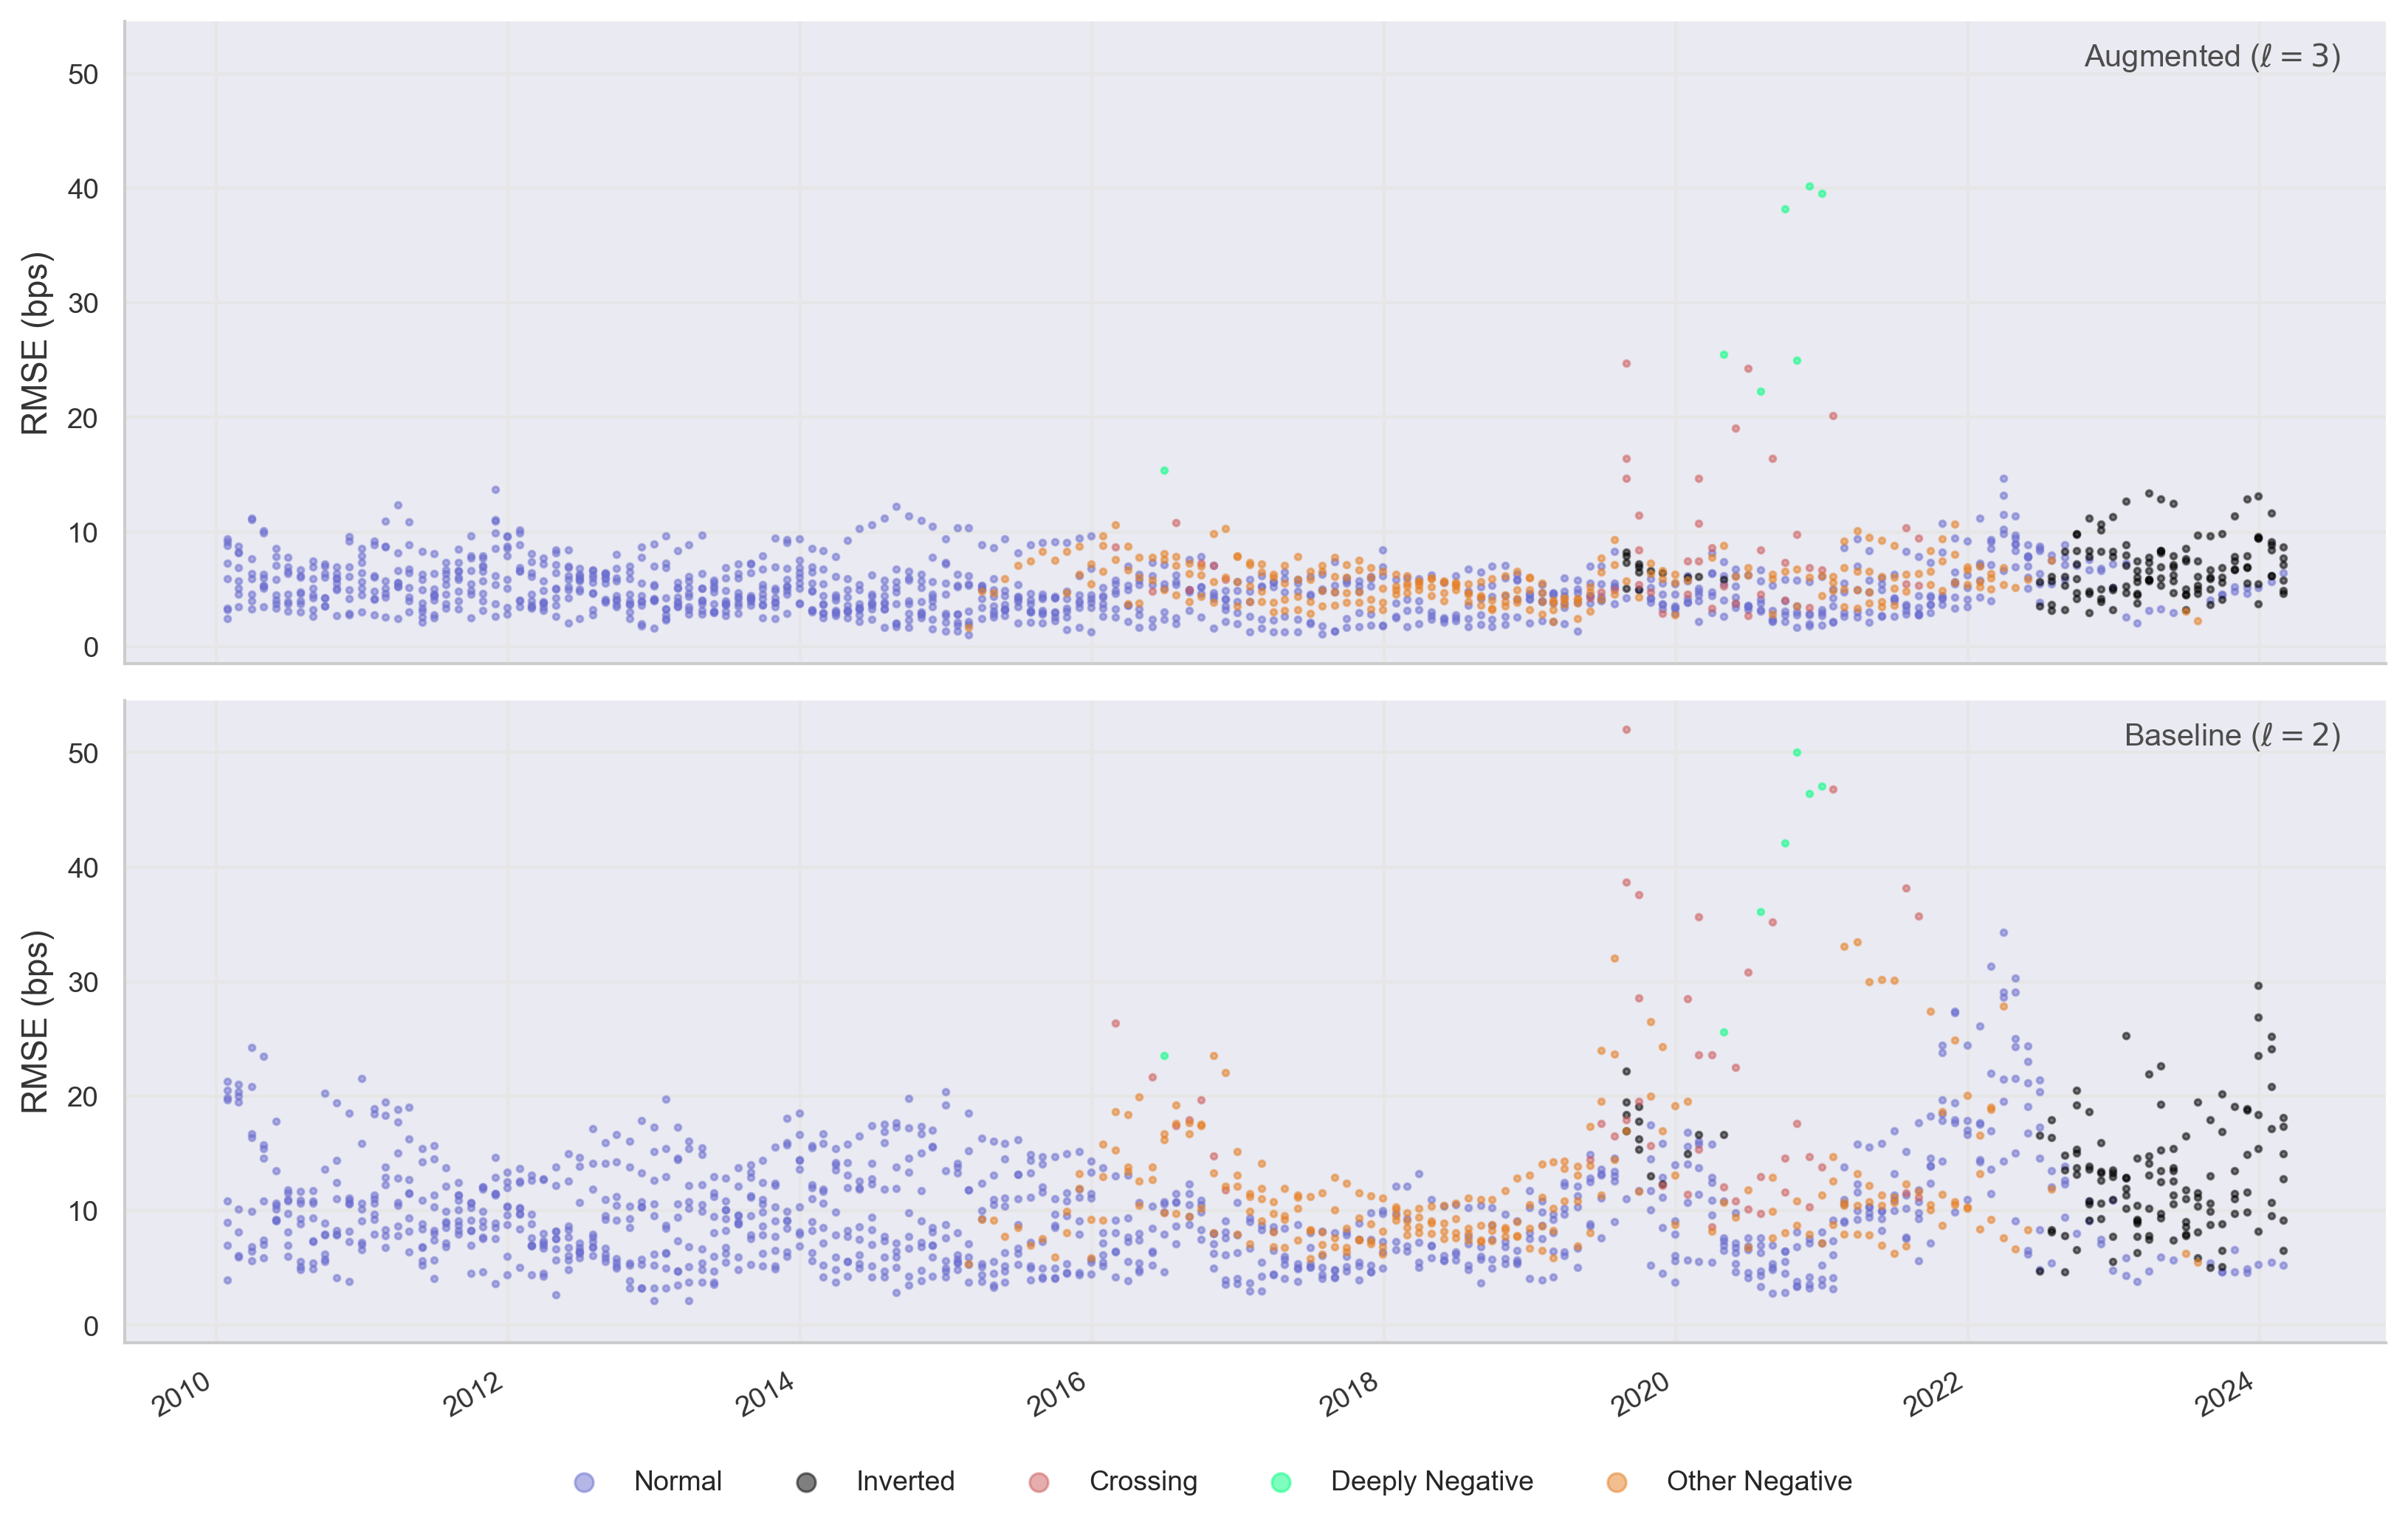
\includegraphics[width=0.95\textwidth]{Figures/thesis_results/AutoencoderPerformanceAugmented/augmented_vs_baseline_is_scatter_dim3.png}
    %\caption{Per-observation in-sample RMSE (bps) over time for the augmented model ($\ell = 3$, top) and the baseline model ($\ell = 2$, bottom). Each point reports the reconstruction error for a single curve observation, coloured by curve type (see Table~\ref{tab:curve_type_counts}). Both panels share the same $y$-axis scale to allow direct comparison between the two models.}
    \caption{Per-observation in-sample RMSE (bps) over time for the augmented model ($\ell = 3$, top) and the baseline model ($\ell = 2$, bottom). Each point reports the reconstruction error for a single curve observation, coloured by curve type. Both panels share the same $y$-axis scale to allow direct comparison between the two models. The augmented model produces a tighter overall error band, with notable reductions for crossing and inverted curves, while deeply negative curves remain challenging for both models.}
    \label{fig:augmented_vs_baseline_is_scatter}
\end{figure}

To assess whether these improvements hold across the full sample rather than only for the selected curves in Figure~\ref{fig:failure_modes_all_models}, Figure~\ref{fig:augmented_vs_baseline_is_scatter} shows that the augmented model with $\ell=3$ latent factors produces lower and more concentrated reconstruction errors than the baseline, particularly for inverted and normal curves. Deeply negative curves remain the most challenging regime for both models, though the augmented model's errors are considerably less severe than the baseline's wrong-direction reconstructions.


As revealed in Figure~\ref{fig:augmented_rolling_regime_dual_axis}, what appears promising in sample does not generalise well out of sample. Despite producing better in-sample reconstructions, the augmented model at $\ell=3$ performs worse out of sample than both the baseline and the augmented model at $\ell=2$. When comparing the two latter, the augmented model $\ell=2$ offers only marginal improvement over the baseline in some periods and worse in others.

To summarise, the augmented model improves in-sample reconstruction for underrepresented curve types, most notably for inverted and crossing curves at $\ell=3$. However, these in-sample gains do not translate out-of-sample, where the augmented model at $\ell=3$ overfits more severely than the baseline, and the augmented model at $\ell=2$ offers only marginal improvement. Augmenting the input representation with explicit shape information is therefore insufficient to improve out-of-sample generalisation for underrepresented curve types.

\begin{figure}[H]
    \centering
    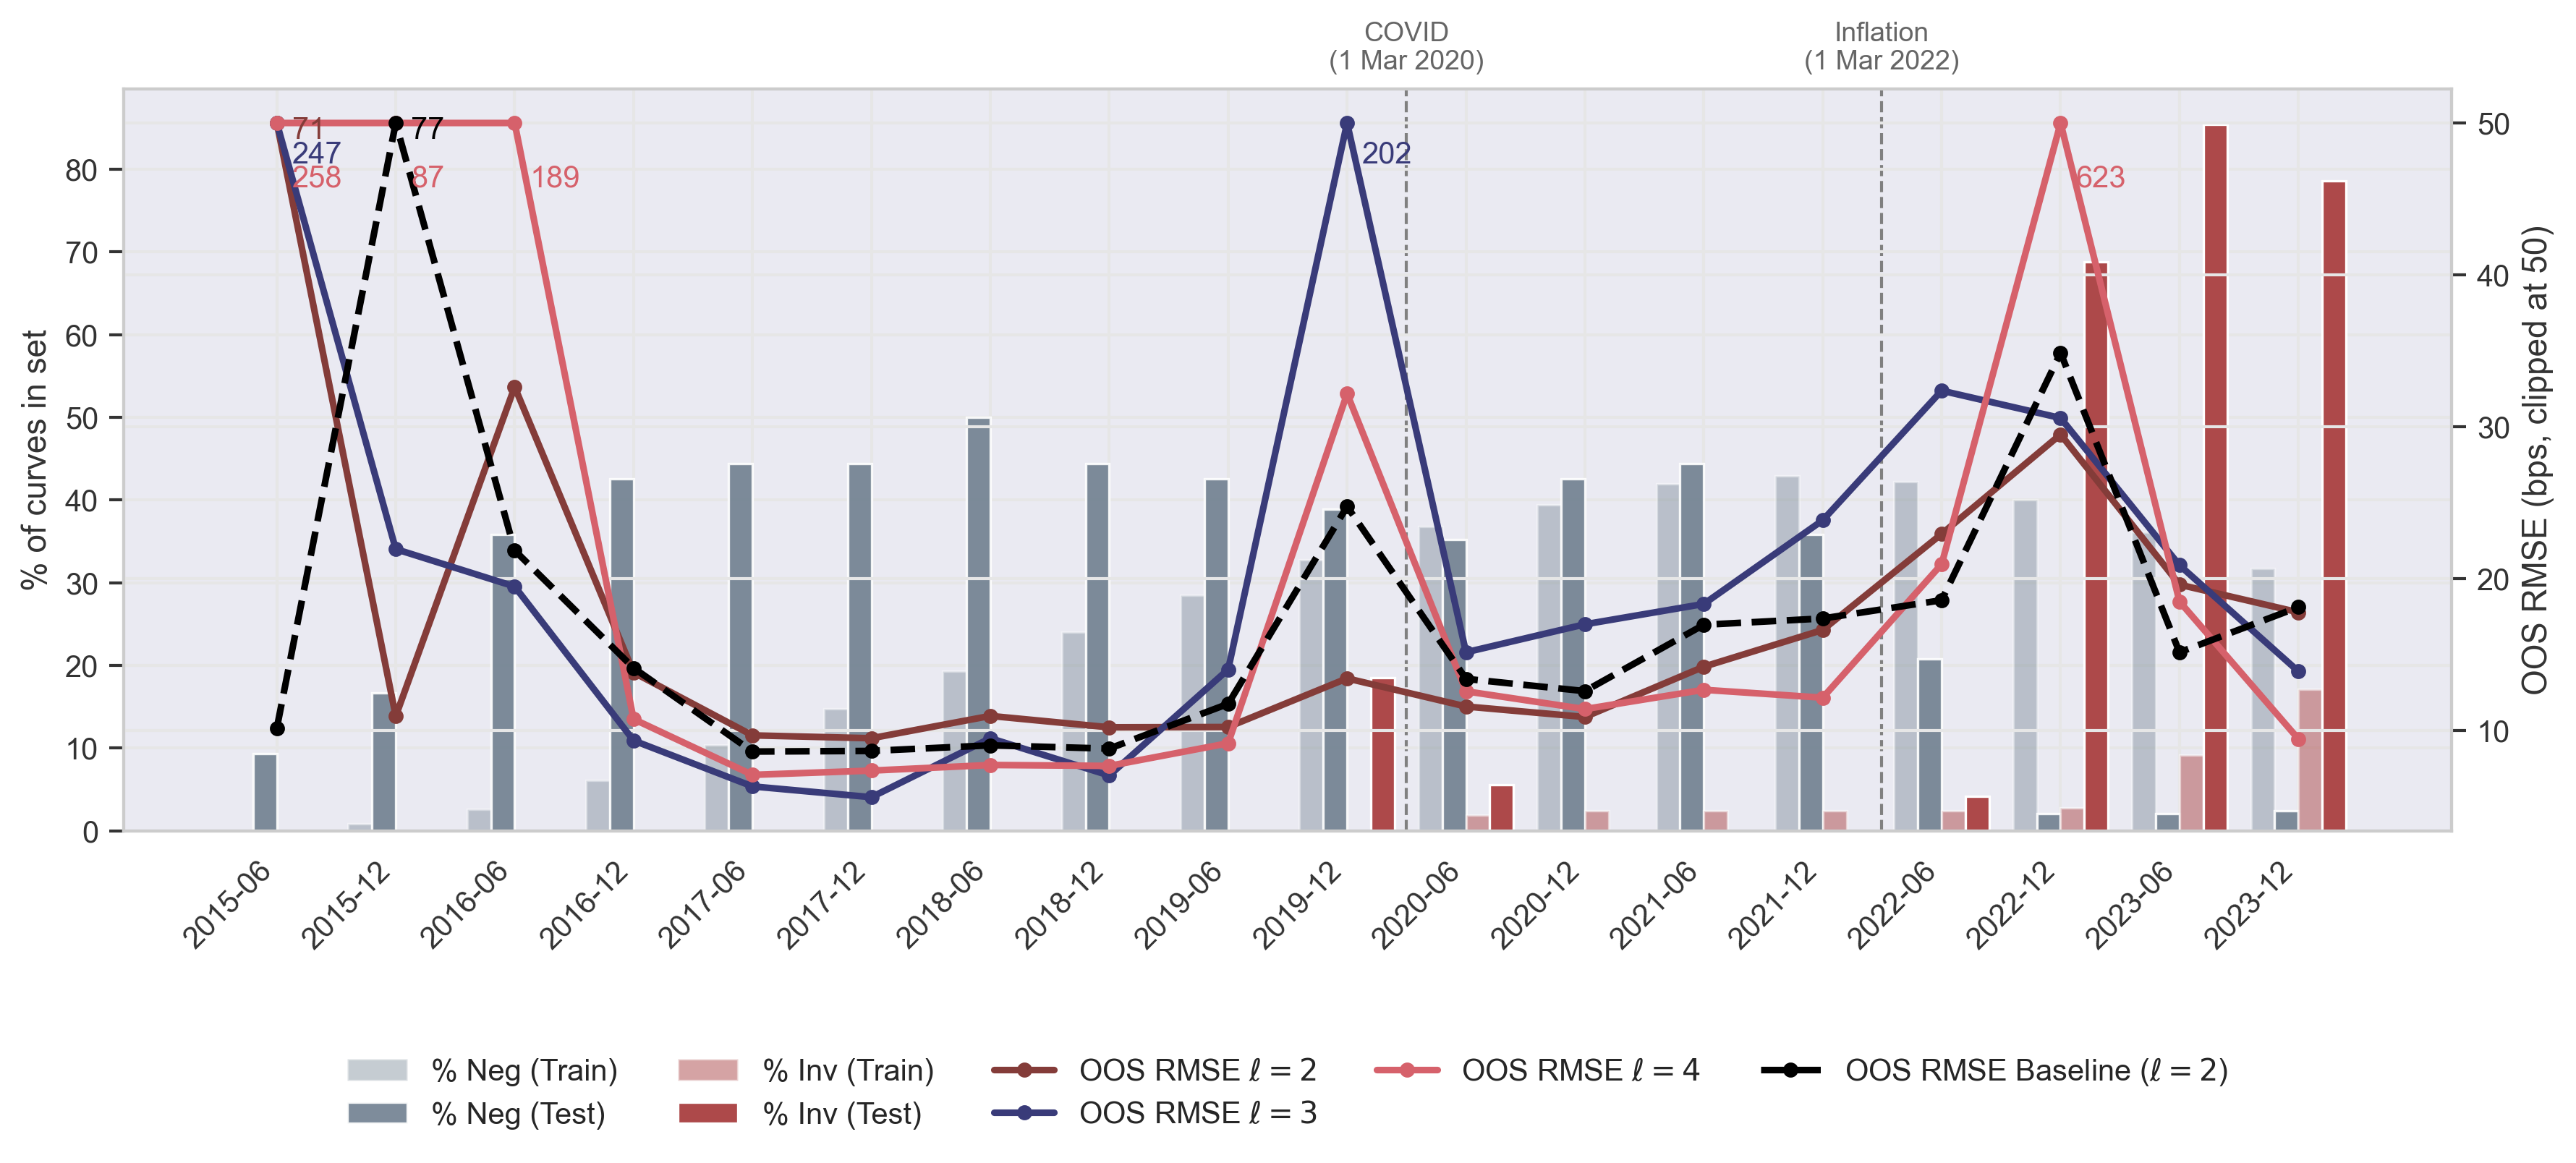
\includegraphics[width=\textwidth]{Figures/thesis_results/AutoencoderPerformanceAugmented/augmented_rolling_regime_dual_axis.png}
    %\caption{Rolling out-of-sample RMSE (bps, right axis) for the augmented model with $\ell \in \{2, 3, 4\}$ latent factors, clipped at 50\,bps. True values are annotated where clipping occurs. The baseline model ($\ell = 2$) is included as a reference (black dashed line). Bars (left axis) show the percentage of negative and inverted curve types in the training and test set of each rolling window. Grey vertical lines mark the onset of macroeconomic regimes.}
    \caption{Rolling out-of-sample RMSE (bps, right axis) for the augmented model with $\ell \in \{2, 3, 4\}$ latent factors, clipped at 50\,bps. True values are annotated where clipping occurs. The baseline model ($\ell = 2$) is included as a reference (black dashed line). Bars (left axis) show the percentage of negative and inverted curve types in the training and test set of each rolling window. Grey vertical lines mark the onset of macroeconomic regimes. The augmented models at \(\ell=3\) and \(\ell=4\) generalise worse out of sample than the baseline, while \(\ell=2\) offers only marginal improvement.}
    \label{fig:augmented_rolling_regime_dual_axis}    
\end{figure}







